\chapter{CASBI: Chemical Abundance Simulation Based Inference}

\section{Simulation Based Inference}
CASBI is a Simulation Based Inference (SBI) package to recover the properties of building blocks of Milky Way like galaxy's halo from observations of the chemical abundance plane. The SBI framework has existed along side the more traditional likelihood based inference methods for quite some years already, and has its root in the Approximate Bayes Computation \cite{rubinBayesianlyJustifiableRelevant1984}, and it has been used in a variety of fields, from cosmology to particle physics. The main difference between SBI and likelihood based methods, like MCMC, is that the former do not require the likelihood function to be known, but rather rely on a simulator to generate synthetic data \textbf{$\mathbf{x}$} once the input parameters $\boldsymbol{\theta}$ are passed to it, and the inference pipeline is trained based on data-parameters pairs ($\mathbf{x}, \boldsymbol{\theta}$). 

Recent advance of this technique was made possible by the use of machine learning models to emulate conditional probability distributions, a technique know as Neural Density Estimation (NDE) \cite{papamakariosNeuralDensityEstimation2019}. The NDE is achieved by training a Normalizing Flow architecture, a generative model that allows to obtain samples from a complex distribution $p(x)$ by constructing a series of \textbf{bijiective} transformations  $f_{\phi_i}^i$ that map $x$ to a latent space $z$ that is distributed as a simple distribution, like a Gaussian. Accordingly to \cite{kingmaGlowGenerativeFlow2018}, implementing the transformations as Neural Network with parameters $\phi_i$, in the end the models learns the following schema:
\begin{equation}
p(x) \sim x \equiv h_0 \xleftrightarrow{\text{$f_{\phi_1}^1$}} h_1 \xleftrightarrow{\text{$f_{\phi_2}^2$}} h_2 \dots \xleftrightarrow{\text{$f_{\phi_K}^K$}} h_K \equiv z \sim \mathcal{N}(z; 0, \mathcal{I}),
\end{equation}
by maximizing the negative log likelihood as loss function and using the change of variable formula as follows:
\begin{equation}
\begin{aligned}
    \text{log} \, p(x) &= \text{log} \, p(z) + \text{log} \left| \text{det} \left( \frac{\partial z}{\partial x} \right) \right| \\
    &= \text{log} \, p(z) + \sum_{i=1}^K \text{log} \left| \text{det} \left( \frac{\partial h_{i}}{\partial h_{i-1}} \right) \right| \\
    &= \text{log} \, p(z) + \sum_{i=1}^K \text{log} \left| \text{det} \left( \frac{\partial f_{\phi_i}^i(h_{i-1})}{\partial h_{i-1}} \right) \right|,
\end{aligned}
\end{equation}
where the last term is the sum of the log determinant of the Jacobian of the transformations $f_{\phi_i}^i$. Once the model is trained it is easy to sample from the distribution $p(x)$ by sampling from the latent space $z$ and applying the inverse transformations $(f_{\phi_1}^1)^{-1} \circ \dots \circ (f_{\phi_K}^K)^{-1}$.
In order to keep the sum of log determinant tractable, the use of \textit{Coupling layers} allows to split the input $x$ along its dimensions and apply a transformation only to a subset of the dimensions, using the other as input for the transformation and keeping it fixed. The subset is than changed at each layers, allowing to have a permutation invariant transformation. The transformations $f^{i}_{\phi_i}$ are usually very simple invertible transformation like a translation and a scaling, or splines functions. 

Following the discussion presented in \cite{hoLtUILIAllinOneFramework2024}, in Bayesian analysis we have the choice to approximate either the Posterior, the Likelihood or the Likelihood ratio, and this choice depend mostly on the problem that one wants to solve. 
\begin{figure}[ht]
    \centering
    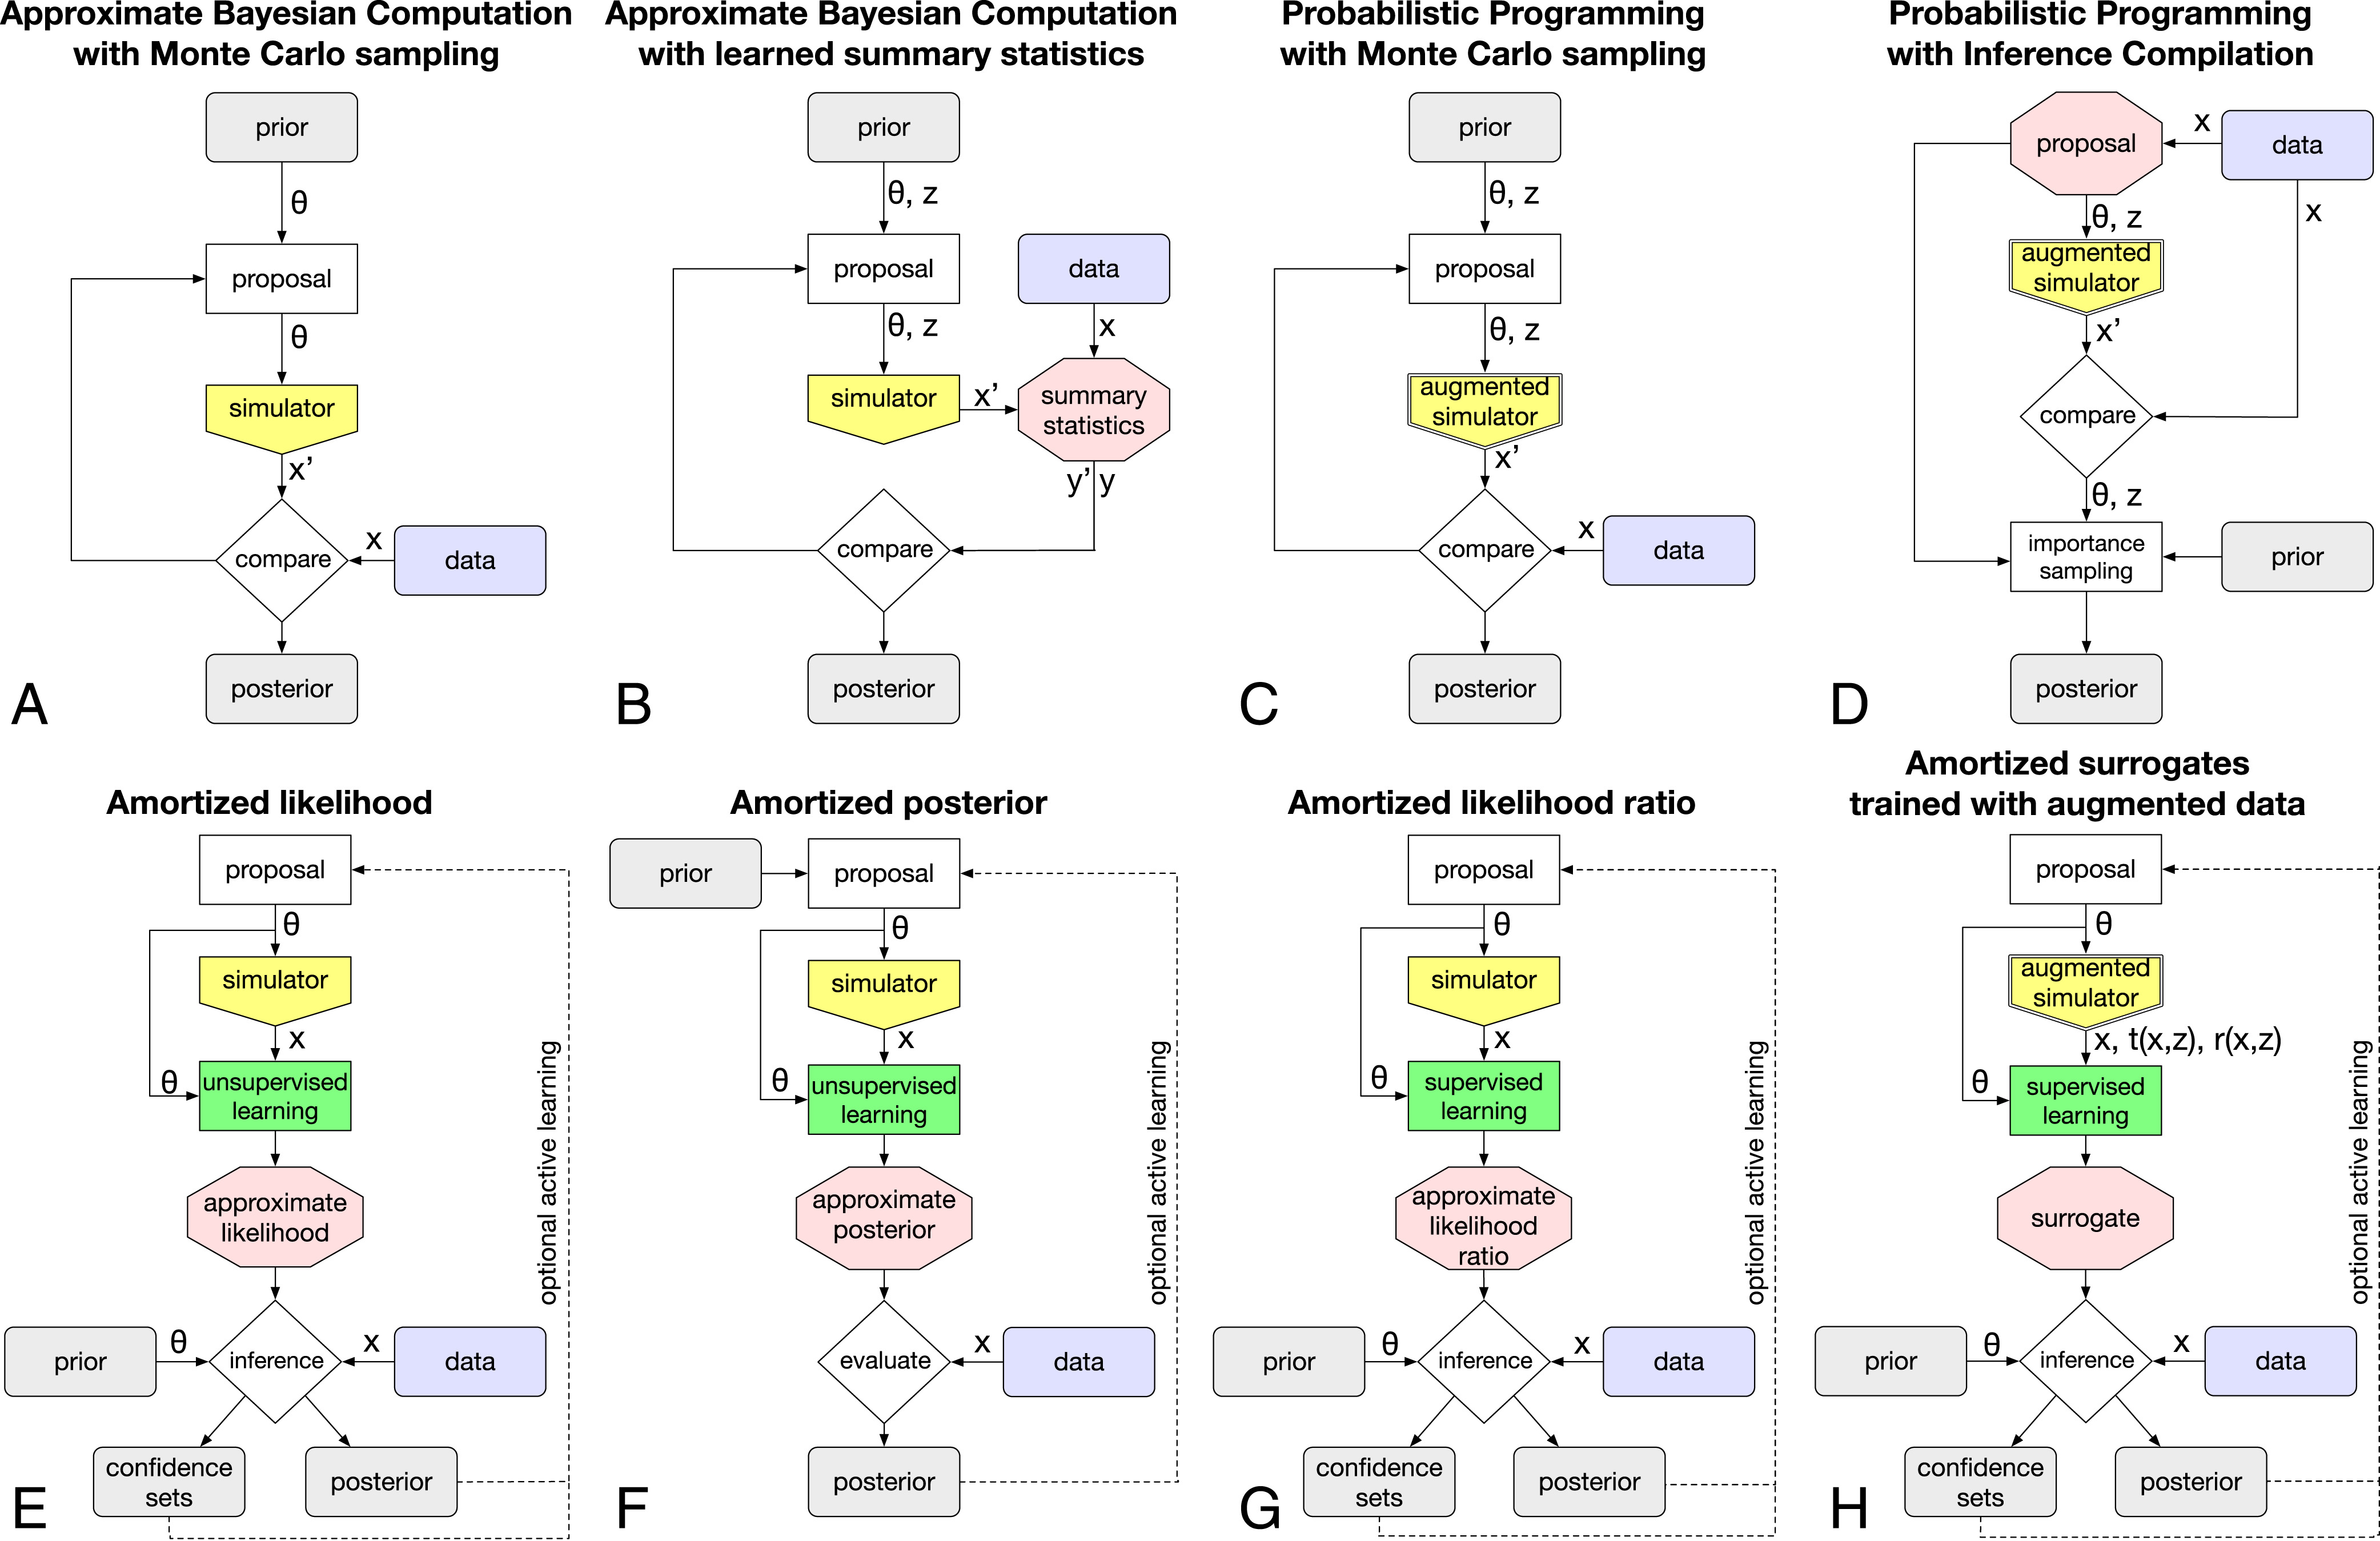
\includegraphics[width=1\textwidth]{./figure/sbi_methods.jpg}
    \caption{Different approaches to Simulation Based Inference, from \cite{FrontierSimulationbasedInference}.}
    \label{fig:sbi_approaches}
\end{figure}

In our case, due to the complexity of the Likelihood distribution of the chemical abundance space, we choose to approximate the Posterior distributions, and so we adopted the Neural Posterior Estimate (method \textbf{F} in Figure~\ref{fig:sbi_approaches}) that can be trained using the negative loglikelihood as loss function:
\begin{equation}
\begin{aligned}
    \mathcal{L}_{NPE}(\boldsymbol{\theta}) &= - \mathbb{E}_{\mathcal{D}_{train}} \text{log} \hat{\mathcal{P}}(\theta_i | x_i) \\ 
    &= - \mathbb{E}_{\mathcal{D}_{train}} \text{log} \left( \frac{p(\theta)}{\tilde{p}(\theta)} q_{\omega}(\theta_i, x_i) \right), 
\end{aligned}
\end{equation}
where our Posterior distribution $ \hat{\mathcal{P}}(\theta_i | x_i)$ is approximated by the product of the ratio of the prior $p(\theta)$ and proposal distribution $\tilde{p}(\theta)$ and the neural conditional distribution $q_{\omega}(\theta_i, x_i)$, parametrized by the parameters $\omega$. 

Many excellent framework for handling SBI analysis are already available, and CASBI is build on top of the \texttt{ltu-ili} python package \cite{hoLtUILIAllinOneFramework2024}. In particular, CASBI analysis were performed relying on the \texttt{sbi} backend \cite{tejero-canteroSbiToolkitSimulationbased2020} to train a \textit{Neural Posterior Estimate}\footnote{The \texttt{sbi} backed implement NPE using \textbf{\texttt{nflows}} \cite{durkanNflowsNormalizingFlows2020}} of the parameters' posteriors. The preprocessing of the data is described in Section~\ref{sec:NIHAO}, the details of the training of the NPE is described in Section~\ref{sec:Two step Inference}.


\section{NIHAO}\label{sec:NIHAO}
The data-parameters pairs $(\mathbf{x}, \boldsymbol{\theta})$ are obtained from the \textbf{NIHAO} project \cite{wangNIHAOProjectReproducing2015}. The \textbf{NIHAO} (Numerical Investigation of a Hundred Astrophysical Objects) is a set of 100 cosmological zoom-in hydrodynamical simulations with halos that range from dwarf ($M_{star} \sim 5 \times 10^9 M_\odot$) to Milky Way like($M_{star} \sim 2 \times 10^{12} M_\odot$). In order to handle these simulations, in CASBI the preprocessing is done with the use of the functions available in \texttt{pynbody} \cite{pontzenPynbodyNBodySPH2013}. In Fig. \ref{fig:NIHAO} we show face on samples of galaxies in the \textbf{NIHAO} simulations set.

\begin{figure}[ht]
    \centering
    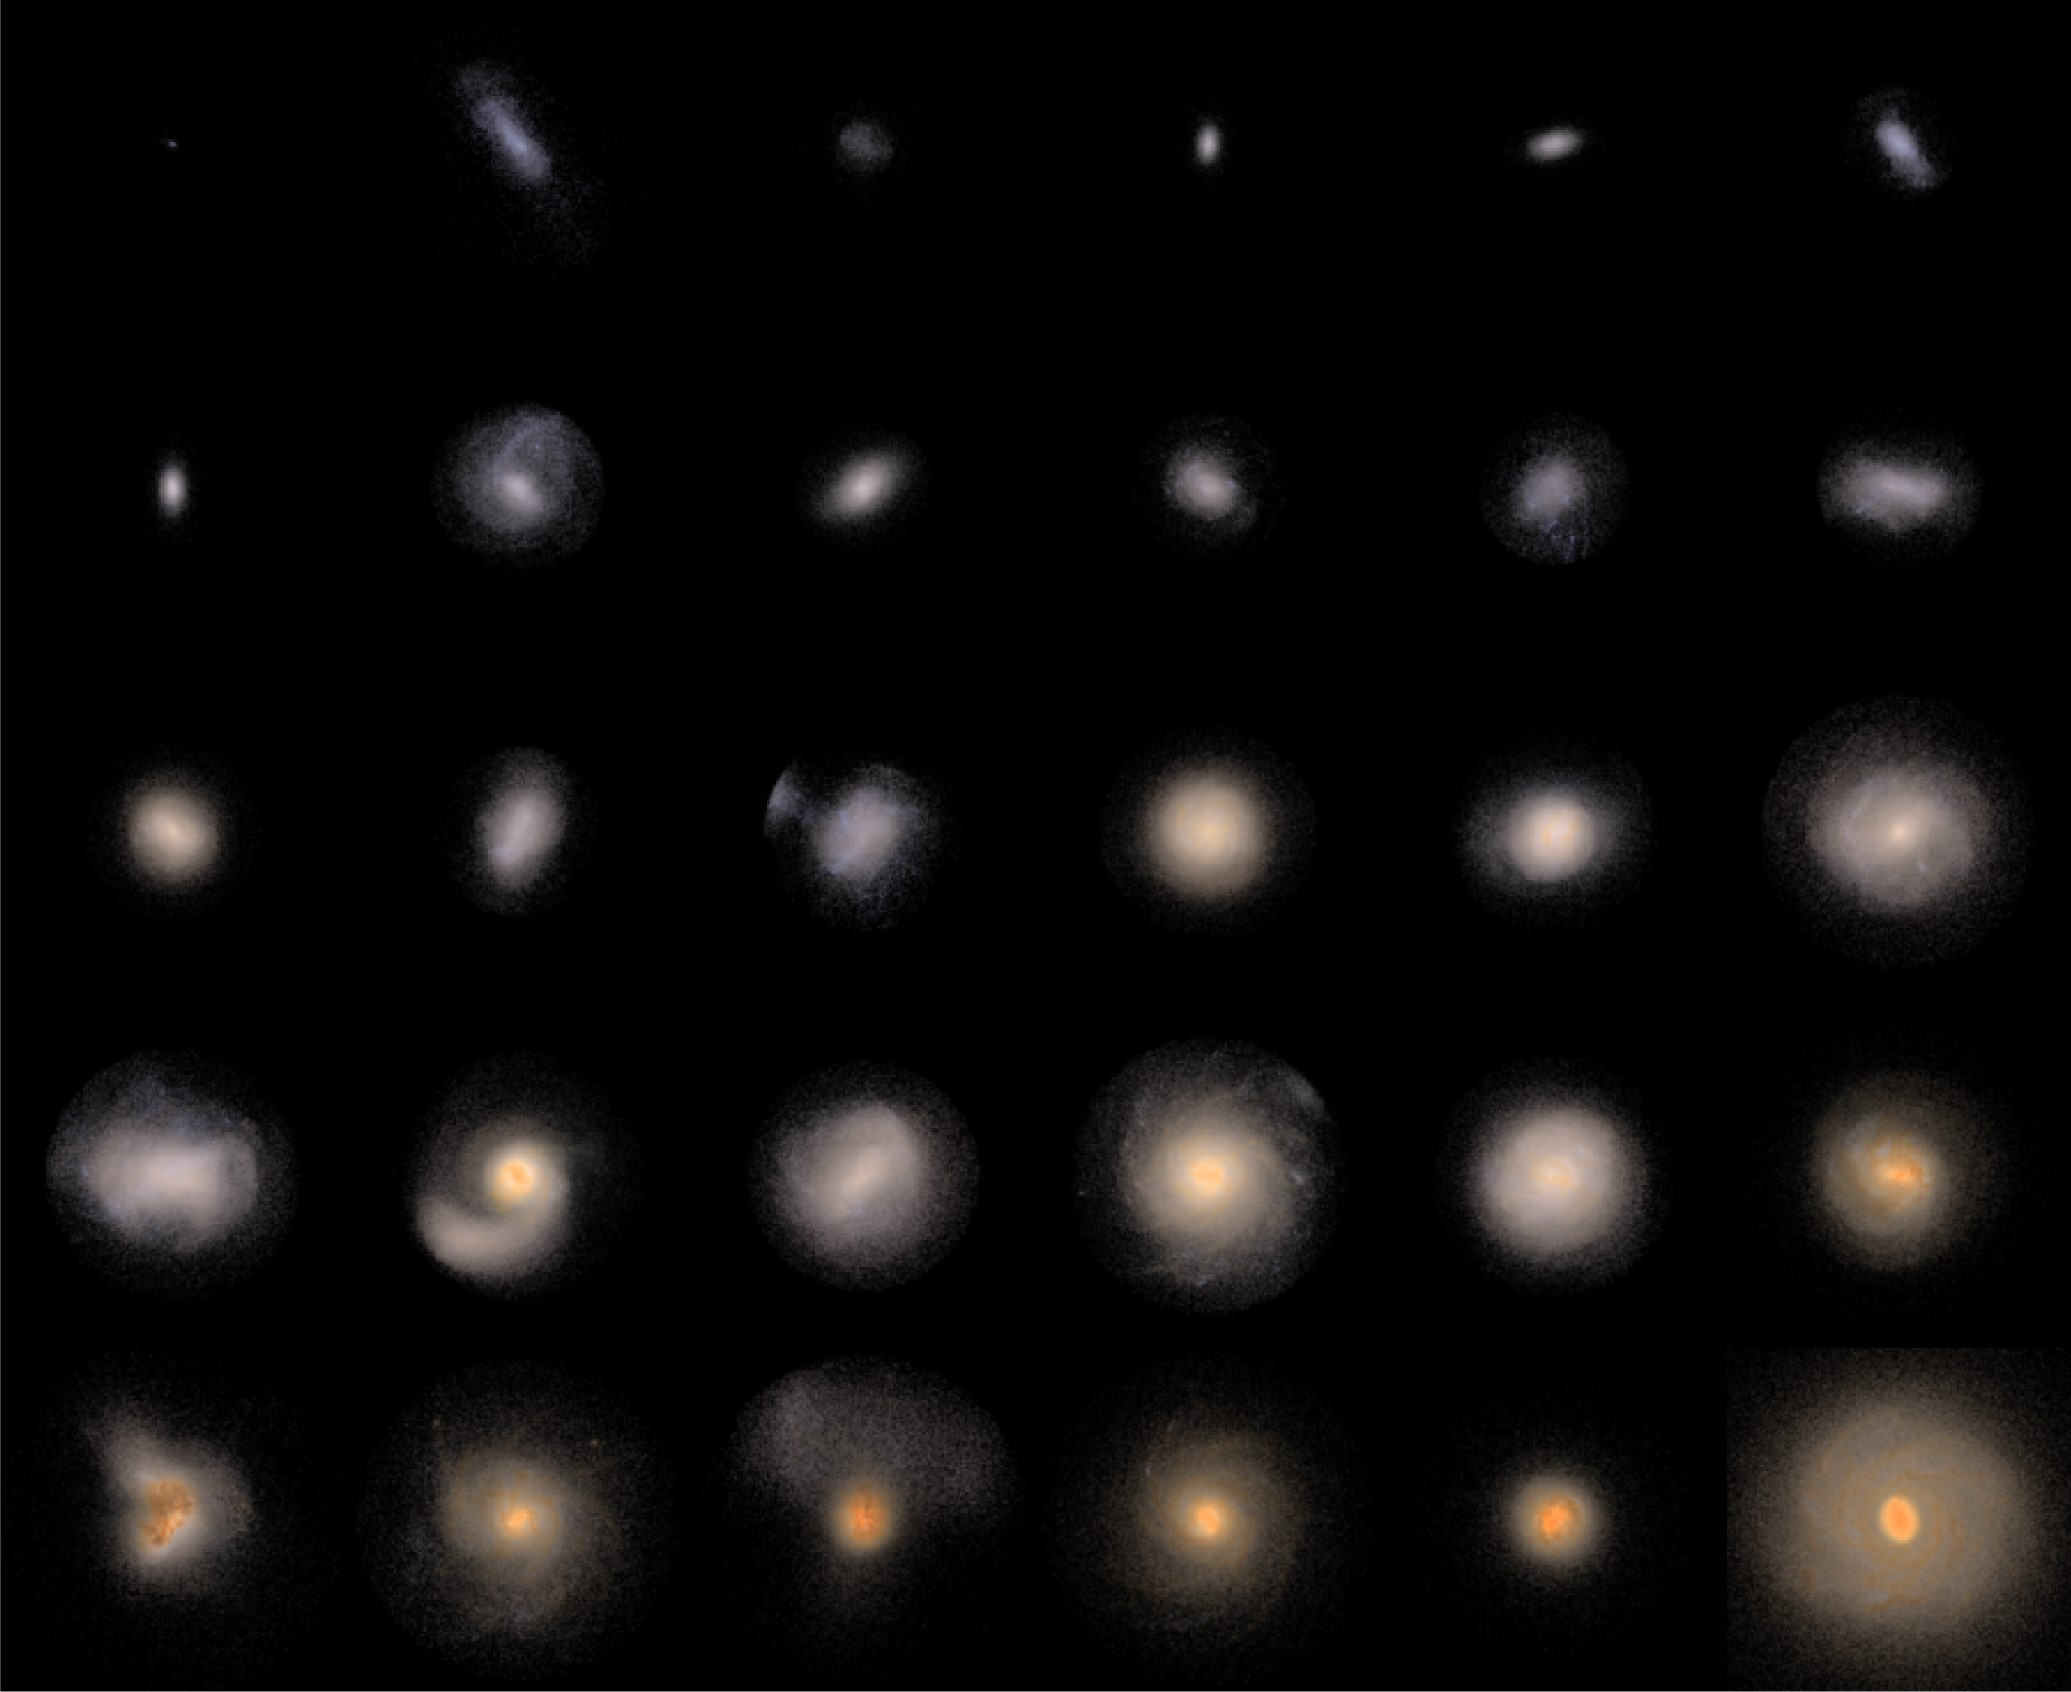
\includegraphics[width=1\textwidth]{./figure/NIHAO.jpeg}
    \caption{Face on \textbf{NIHAO} galaxies from \cite{wangNIHAOProjectReproducing2015}.}
    \label{fig:NIHAO}
\end{figure}

Similarly to \cite{cunninghamReadingCARDsImprint2022} and \cite{deasonUnravellingMassSpectrum2023}, we rely on the assumption that once the accreted object falls into the gravitational potential of the Milky Way like galaxy its star formation rate is halted, so we can treat each of the snapshot in this simulations as a possible building block of galactic halo. In order to create observables we construct 2D histogram, referred to as \textbf{$\mathbf{x^i}$}, of counts of the chemical abundance plane $[O/Fe]$ over $[Fe/H]$ ($\alpha$ element abundance over metallicity) for each of the snapshot available in \textbf{NIHAO}, after filtering in order to have galaxies with a total stellar mass $M_{star} < 6 \times 10^9 M_\odot$, which is the stellar mass of the Large Magellanic Cloud, the largest accreted object by the Milky Way. These 2D histogram have $64 \times 64$ pixels, they have minimum and maximum values set after filtering all the stars that were outside the 0.01 percentile in either metallicity or $\alpha$ element abundance, and they are linked to galaxy snapshot trough the \texttt{Galaxy\_name} attribute. The actual observable \textbf{$\mathbf{x^j} = \sum_i^{N_{sub}^j} x^j_i$ } used in CASBI is then a super imposition of $N_{sub}$ of these 2D histograms, where the $N_{sub}^j$ is the number of accreted objects present in the $j$-th galaxy halo. In CASBI the inference is done on two set of parameters, the $N_{sub}^j$ and the \textbf{$\mathbf{\theta^j}$} = ($M_{star, i}^j, M_{dm, i}^j, \tau_i^j $) with $i=2, ..., N_{sub}$, which are respectively the total stellar mass, the total dark matter mass, and the infall time (in Gyr) of the $i$-th accreted object in the $j$-th sample. The inference pipeline is further described in  the following section.
  
\section{Two step Inference}\label{sec:Two step Inference}
The objective of the inference is not trivial, since in order to recover the parameters of the building blocks of the Milky Way like galaxy we need to fix the dimensionality of the priors. This is equivalent to have complete knowledge on the number of substructure that are present in the galactic halo. In the case of not fully phase mixed structure, the dynamical information could be use to help to disentangle this structure, and also to separate them from the host halo background. In CASBI we do not leverage on this information because it would require to construct stellar halo that have aggregated objects that are not dynamically biased. We leave this integration for future work. We decided to tackle this problem in the case of fully mixed remnants separating the inference in two steps:
\begin{enumerate}
    \item \textbf{Inference of the number of substructure}: In this step we train a NPE to recover the posterior distribution of the number of substructure $N_{sub}$, by using the observable \textbf{$\mathbf{x^j}$}. The prior for the parameter is assumed to be uniform between 2 and 100. This boundaries were selected in accordance to the order of magnitude of substructures found in \cite{deasonUnravellingMassSpectrum2023}. For each of the possible $N_{sub}$ we extract 1000  $x^j = \sum_{i=1}^{N_{sub}} x_i^j$ from the \textbf{NIHAO} simulations, in order to have a total of almost $ 10^5$ sbi training couples $(N_{sub}^j, x^j)$, with 20 \% used as validation, and we use the same process to generate almost $10^4$ test set samples, making sure that the same combinations of \texttt{Galaxy\_name} attribute weren't shown in training and test. The training of the NPE is done using the \texttt{sbi} backend, using 4 \texttt{nsf} (neural spline flow) with 10 layers and 100 neurons each. In order to take full advantage of the image-like structure of the data, we adopt as embedding network a Convolutional Neural Network (CNN) to reduce the dimensionality of the input of the NPE from $64 \times 64$ to 128. 
    In this step we have not impose that the $N_{sub}$ must be a discrete variable, and we have decide to just truncate the inferred value to the closet value. To the knowledge of the author no SBI framework has implemented a way of dealing with the inference of discrete random variables, so we leave a more precise implementation as a future work. We propose instead another method to obtain the number of substructure, by casting this inference as a classification problem. We use a SkipConnection CNN, considering the number of substructure as the label to assign to each $x^j$.

    \item \textbf{Inference of $\mathbf{\theta^j}$}: Once we have the estimate $\tilde{N}_{sub}$, whether using dynamical information, or the inference pipeline or the classification method, we can proceed to the inference of the parameters $\mathbf{\theta^j}$. The prior for the parameters are assumed to be uniform between the minimum and maximum values available for the galaxies that we have filtered from the NIHAO simulations. We extract $10^5$ random samples of $\tilde{N}_{sub}$ snapshots from the \textbf{NIHAO} simulations, and we construct the observable 
    couples $(x^j, (\theta_1^j, \dots, \theta_{\tilde{N}_{sub}}^j))$, with 20 \% used as validation and the rest as training. We repeat the same process to generate $10^3$ test set samples, making sure that the same combinations of \texttt{Galaxy\_name} attribute weren't shown in training and test to perform calibration of the inference model. The training of the NPE is done using the \texttt{sbi} backend, using 4 \texttt{nsf} (neural spline flow) with 10 layers and 100 neurons each. Once again we use a CNN as embedding for our observation $x^j$.
\end{enumerate}

% The analysis with this two step inference did not satisfy the author, because the inference on the number of subhalos, or the classification, was not accurate enough to be generate a good foundation for the prior distribution of the second step. The inference pipeline for the parameters $\mathbf{\theta^j}$ did not converge using the fast \texttt{direct sampling}. This could happen because the Normalizing flow architecture do not constrain the support of the posterior, and the inference could get stack because the sampling happens in region outside the boundaries of the prior distribution. In order to overcome this limitation one might decide to switch to a traditional MCMC sampler, but due to the time consuming nature of this method we decided to rethink the inference pipeline, presented in the next subsection.    

\section{Realistic halo and 1 step Inference}

\begin{figure}[ht]
    \centering
    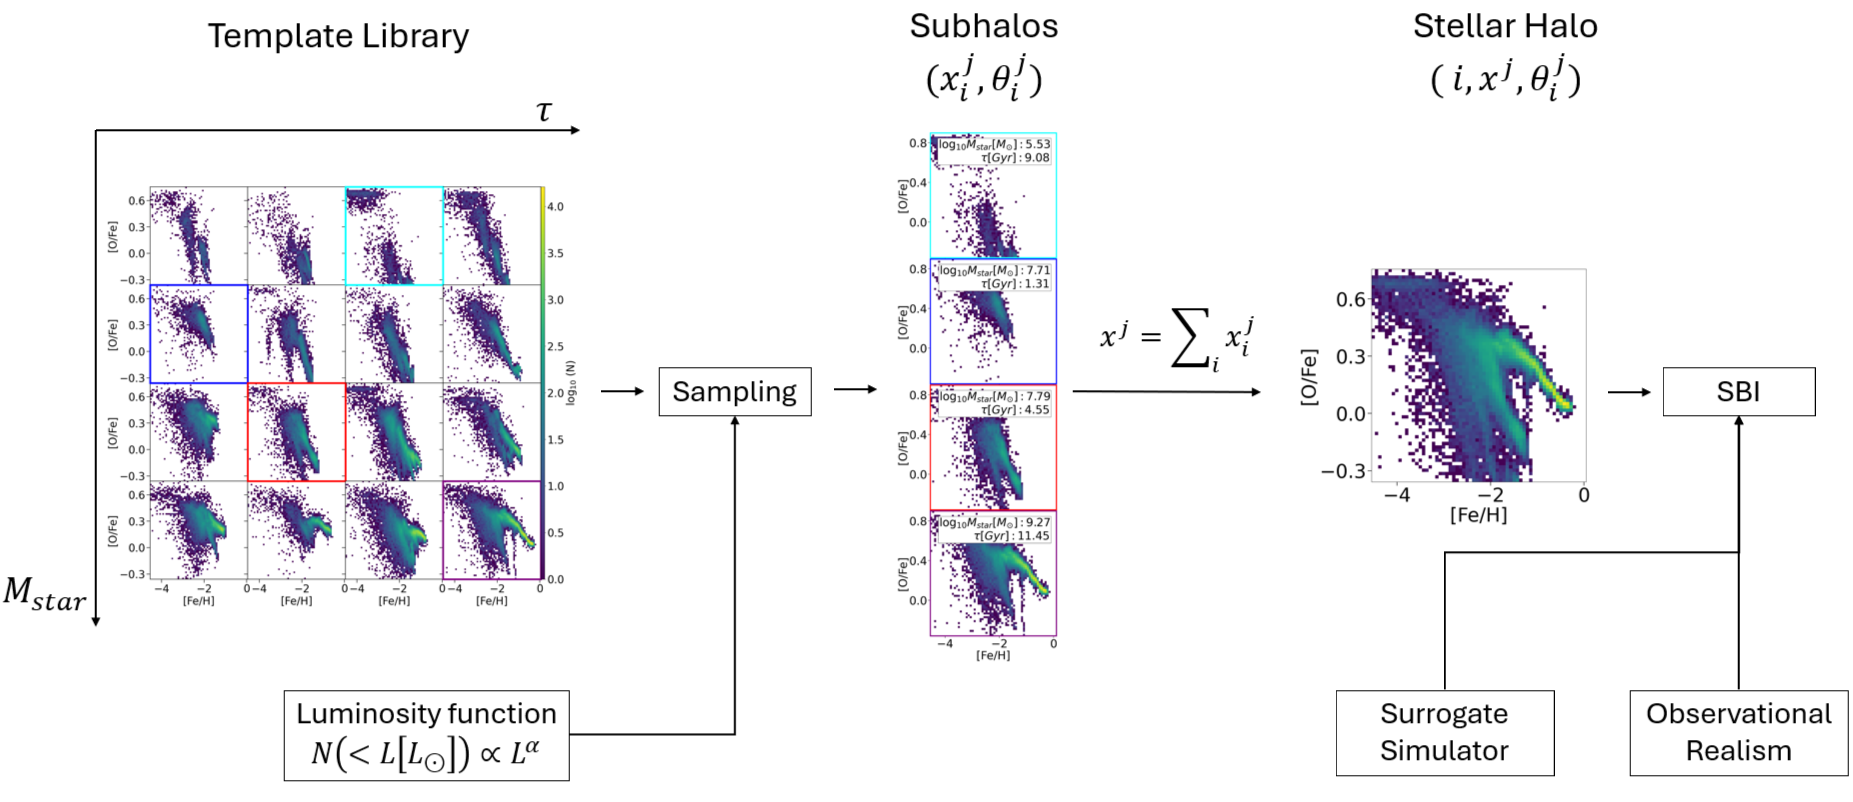
\includegraphics[width=1\textwidth]{./figure/CASBI.png}
    \caption{CASBI pipeline.}
    \label{fig:CASBI}
\end{figure}

In order to avoid the need for a two step inference and still retaining the possibility to access to the information on how many subhalos populate a given abundance plane, we have decided to condition the SBI model to retrieve the $i$-most massive subhalo of the $j$-th stellar halo. In this way the NPE is trained on $(x, \theta) = (i, x^j, \theta_i^j)$ pairs, where $x^j = \sum_i x_i^j$ and the $x_i^j$ are ordered accordingly to their stellar mass. In this way the $j$-th stellar halo abundance plane is shown as many times as the number of subhalos present in it, so in order to guide the model into inferring the right parameters $\theta_i^j$ the embedding is conditioned on the integer $i$-th by concatenating it to each input of the fully connected layers of the CNN used to embed the observations, and it is concatenate also before passing the embedded information to the Normalizing Flow. 

In order to be more realistic in the creation of a mock galaxy halo we have decided to adopt a sampling scheme for the subhalos that is based on the luminosity function described in \cite{koposovLuminosityFunctionMilky2008}. The luminosity function described the subhalo distribution in a range of luminosities that spans from $M_V = -2$ all the way to the luminosity of the Large Magellanic cloud:
\begin{equation}
    \frac{dN}{d M_V} = 10 \times 10^{0.1(M_V + 5)} 
\end{equation}
we can then manipulate this equation to express it as a function of the Luminosity in solar luminosity $L$:
\begin{equation}
\begin{split}
    \frac{dN}{dL} &= \frac{dN}{d M_V} \times \frac{dM_V}{dL} \\
    &= 10 \times 10^{0.1(M_V + 5)} \times 0.4 \times 10^{0.4(M_{V, \odot} - M_V)} \\
\end{split}
\end{equation}

which in the end can be integrated to obtain the number of subhalos with luminosity lower the $L$ that we are going to adopt for sampling stellar halo:
\begin{equation}
    N(<L) = K \times L^{\alpha},
\label{eq:CumLuminosity}
\end{equation}
where K represent a constant and $\alpha=-1.25$ is the single power law exponent obtained by \cite{koposovLuminosityFunctionMilky2008}. Other work based not only on SDSS observations like \cite{koposovLuminosityFunctionMilky2008} but also on $\Lambda$CDM $N$-body simulation set $\alpha = -1.9 \pm 0.2$ (\cite{tollerudHundredsMilkyWay2008}). We fix this value to -1.25 and we leave the analysis of the impact of this choice as a future work.
Assuming $L_\odot = M_\odot$, we normalize equation \ref{eq:CumLuminosity} after setting the support to be the interval of masses that we have available in our catalogue of NIHAO simulations ($10^5 M_\odot < M < 6 \cdot 10^9 M_\odot$) and we sample from this distributions using an inverse scheme. After obtaining the analytic samples we take the first and second Nearest Neighbors (NN) that are within a  
10\% of the analytic sampled mass as subhalo for our mock halos. We have also set a mass budget for our mock halo of $M=1.4 \pm 0.2 \times 10^9 M_\odot$ based on \cite{deasonTotalStellarHalo2019}, and each time a subhalo is sampled we reduce the total mass budget by the mass of the NN that we have used. We decision to put a total mass halo was made in order to avoid to set a fixed number of subhalos that needs to be sampled for each stellar halo. During this iterative procedure we make sure to sample non repeated subhalo within the same mock halo and we avoid repetitions of the same combinations of subhalos between mock subhalos both within training and test set and across these two sets.

In Fig. \ref{fig:CASBI} we show the CASBI pipeline. The modularity of the SBI technique is fully integrated, allowing to change all the components of this pipeline. The Template library can be set to be a different any kind of suite of simulated galaxies (e.g. \cite{pillepichMilkyWayAndromeda2023}), the sampling scheme can incorporate different luminosity function and stellar halo budget, the NPE and embedding network architecture and hyperparameter can be modified to allow for higher accuracy and posterior coverage thanks to the \texttt{optuna} grid search implementation, and surrogate models (Free Form Flow FFF \cite{draxlerFreeformFlowsMake2024}, GRUMPY \cite{kravtsovGRUMPYSimpleFramework2022}) can be implemented to allow for the sequential version of the NPE.      


\section{Free Form Flow as a surrogate simulator}


